\documentclass{beamer}

\usepackage{graphicx}
\usepackage{textpos}
\usepackage{listings}
\usepackage{lstautogobble}

\usetheme{Madrid}
\useoutertheme{miniframes} % Alternatively: miniframes, infolines, split

% Setup the university's color pallette
\definecolor{UIUCorange}{RGB}{19, 41, 75} % UBC Blue (primary)
\definecolor{UIUCblue}{RGB}{232, 74, 39} % UBC Grey (secondary)

\definecolor{codegreen}{rgb}{0,0.6,0}
\definecolor{codegray}{rgb}{0.5,0.5,0.5}
\definecolor{codepurple}{rgb}{0.58,0,0.82}
\definecolor{backcolour}{rgb}{0.95,0.95,0.92}

\lstdefinestyle{python}{
  backgroundcolor=\color{backcolour},   
  commentstyle=\color{codegreen},
  keywordstyle=\color{magenta},
  numberstyle=\tiny\color{codegray},
  stringstyle=\color{codepurple},
  basicstyle=\ttfamily\footnotesize,
  breakatwhitespace=false,         
  belowskip=-0.5em,
  breaklines=true,                 
  captionpos=b,                    
  keepspaces=true,                 
  %numbers=left,                    
  numbersep=5pt,                  
  showspaces=false,                
  showstringspaces=false,
  showtabs=false,                  
  tabsize=2
}

\lstset{style=python}

\AtBeginSection[]{
  \begin{frame}
    \vfill
    \centering
    \begin{beamercolorbox}[sep=8pt,center,shadow=true,rounded=true]{title}
      \usebeamerfont{title}\insertsectionhead\par%
    \end{beamercolorbox}
    \vfill
  \end{frame}
}
% Setup the university's color pallette
\definecolor{UIUCorange}{RGB}{19, 41, 75} % UBC Blue (primary)
\definecolor{UIUCblue}{RGB}{232, 74, 39} % UBC Grey (secondary)


\setbeamercolor{palette primary}{bg=UIUCorange,fg=white}
\setbeamercolor{palette secondary}{bg=UIUCblue,fg=white}
\setbeamercolor{palette tertiary}{bg=UIUCblue,fg=white}
\setbeamercolor{palette quaternary}{bg=UIUCblue,fg=white}
\setbeamercolor{structure}{fg=UIUCorange} % itemize, enumerate, etc
\setbeamercolor{section in toc}{fg=UIUCblue} % TOC sections

\setbeamercolor{subsection in head/foot}{bg=UIUCorange,fg=UIUCblue}
\setbeamercolor{subsection in head/foot}{bg=UIUCorange,fg=UIUCblue}

\usepackage[utf8]{inputenc}
\usepackage{graphicx}

%Information to be included in the title page:
\title{\textbf{Adv. Functions}}
\author{\textbf{David H Smith IV}}
\institute[\textbf{UIUC}]{\textbf{University of Illinois Urbana-Champaign}}
\date{\textbf{Tues, Nov 16 2021}}

\setbeamertemplate{title page}[default][colsep=-4bp,rounded=true]
\addtobeamertemplate{title page}{\vspace{3\baselineskip}}{}
\addtobeamertemplate{title page}{
  \begin{textblock*}{\paperwidth}(-1.0em, -1.2em)
    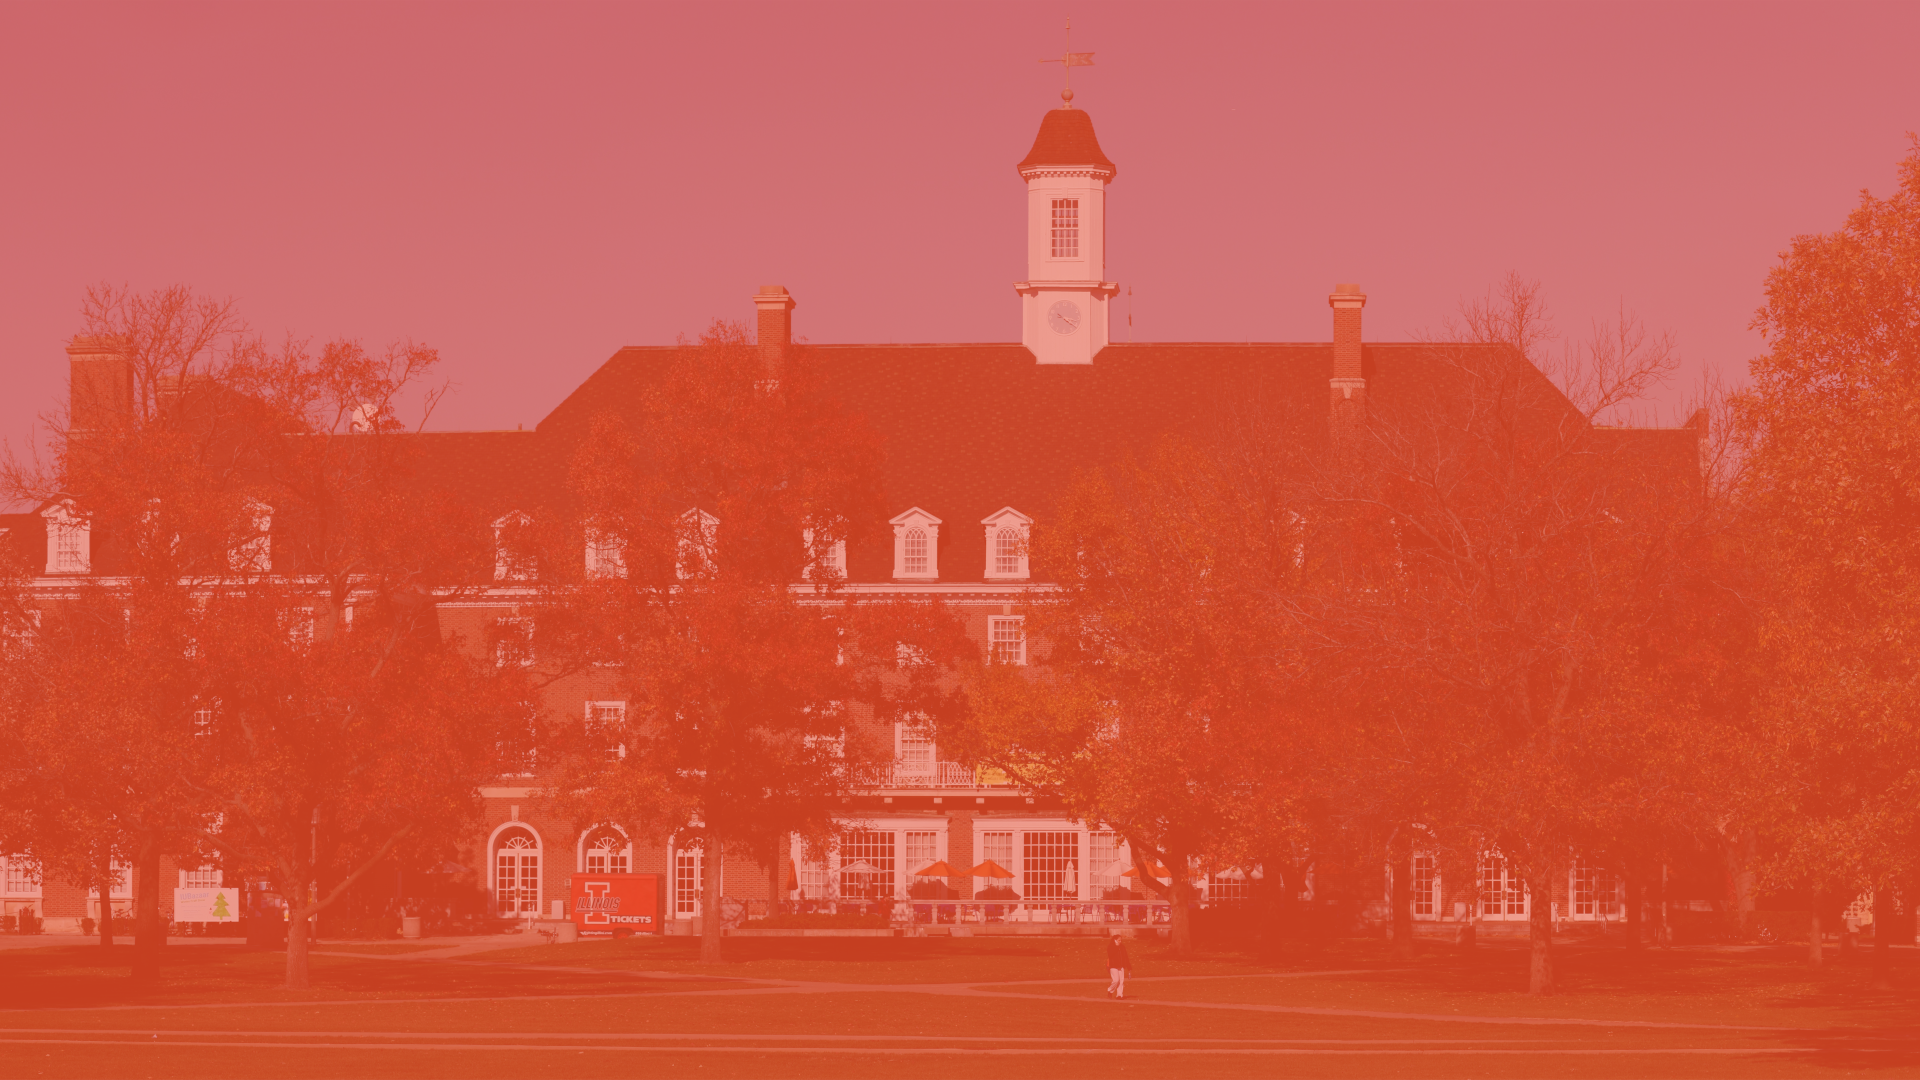
\includegraphics[width=\paperwidth, height=\paperheight]{imgs/uiuc.png}
  \end{textblock*} 
}{}

\begin{document}

\frame{\titlepage}

\section{Course Overview}

%
% Slide 1
%
\begin{frame}
  \frametitle{Reminders}
  \begin{itemize}
    \item Things are due. Check the calendar.
  \end{itemize}
\end{frame}

\section{}

%
% Slide 2
%
\begin{frame}[fragile]
  \frametitle{Bytecode: Looking under the hood}
  \textbf{Python code:}\\
  \begin{lstlisting}[language=Python, autogobble]
  def hello():
      print("Hello, World!")
  \end{lstlisting}
  \vfill
  \textbf{Bytecode:}\\
  \begin{lstlisting}[language=Python, autogobble]
              0 LOAD_GLOBAL              0 (print)
              2 LOAD_CONST               1 ('Hello, World!')
              4 CALL_FUNCTION            1
              6 POP_TOP
              8 LOAD_CONST               0 (None)
             10 RETURN_VALUE
  \end{lstlisting}
  \vfill
  \begin{enumerate}[A]
    \item The computer doesn't just read the code you write.
      \pause
    \item Python is a (kinda) interpreted language: source.py \textrightarrow \ bytecode.pyc \textrightarrow \ interpreter
      \pause
  \end{enumerate}
\end{frame}

%
% Slide 2
%
\begin{frame}[fragile]
  \frametitle{Bytecode: Looking under the hood}
  You can view the bytecode of any function via the following:
  \begin{lstlisting}[language=Python, autogobble]
  import dis

  def hello():
    print("Hello, World!")

  dis.dis(hello)
  \end{lstlisting}
  \vfill
  \begin{enumerate}[A]
    \pause
    \item Compiled vs Interpreted:
      \begin{enumerate}
        \pause
      \item \textbf{compiled} \textrightarrow \ Convert source code into another language. Typically, though not exclusively, a higher level language (e.g., Python) into a lower level language (e.g., bytecode).
        \pause
        \item \textbf{interpreted} \textrightarrow \ Another program reads the code you wrote one line at a time and performs those operations.
      \end{enumerate}
    \pause
    \item There's generally crossover between these.
    \pause
    \item Why bother? Because interpreting bytecode is faster.
  \end{enumerate}
\end{frame}

\section{Functions are Objects}

%
% Slide 2
%
\begin{frame}[fragile]
  \frametitle{Poll Question: Functions}
  What, if anything, gets printed to the screen after this code executes?
  \begin{lstlisting}[language=Python, autogobble]
  def add1(x): return x + 1
  def mul2(x): return x * 2

  x = 1
  fns = [add1, mul2, mul2, print]
  for f in fns:
    x = f(x)
  \end{lstlisting}
  \vfill
  \begin{enumerate}[A]
    \item 1
    \item 4
    \item 8
    \item SyntaxError
  \end{enumerate}
\end{frame}

%
% Slide 2
%
\begin{frame}[fragile]
  \frametitle{Functions are Objects}

  \begin{lstlisting}[language=Python, autogobble]
  def foo(arg1, arg2):
    if arg1 == arg2:
      return "They're equal"
    return "They're not equal"
  \end{lstlisting}
  \vfill
  \begin{itemize}
    \pause
    \item \lstinline|foo.__doc__| \textrightarrow \ The docstring for the function.
    \pause
    \item \lstinline|foo.__code__| \textrightarrow \ Gives the address of the code portion of the foo object in memory.
      \begin{itemize}
        \pause
        \item \lstinline|foo.__code__.co_argcount| \textrightarrow \ The number of arguments in the function object.
        \pause
        \item \lstinline|foo.__code__.co_consts| \textrightarrow \ The literals present in the function object.
        \pause
        \item \lstinline|foo.__code__.co_name| \textrightarrow \ The name of the function.
        \pause
        \item \lstinline|foo.__code__.co_varnames| \textrightarrow \ A tuple of the names of variables present in the function object.
      \end{itemize}
  \end{itemize}
\end{frame}

\section{Namespace}

%
% Slide 2
%
\begin{frame}[fragile]
  \frametitle{Namespace}
  \begin{minipage}{0.49\textwidth}
    \begin{lstlisting}[language=Python, autogobble, basicstyle=\tiny]
      print('Initial global namespace: ')
      print(globals())

      my_var = "This is a variable"
      print('\nCreated new variable')
      print(globals())

      def my_func():
          pass

      print('\nCreated new function')
      print(globals())
    \end{lstlisting}
  \end{minipage}
  \begin{minipage}{0.49\textwidth}
    \begin{lstlisting}[language=Python, autogobble, basicstyle=\tiny]
      Initial global namespace: 
      {}

      Created new variable
      {'my_var': 'This is a variable'}

      Created new function
      {'my_func': <function my_func at 0x2349d4>, 'my_var': 'This is a variable'}
    \end{lstlisting}
  \end{minipage}
  \vfill
  \begin{enumerate}
    \item Maps names to objects.
    \pause
    \item You can check the local namespace with \lstinline|locals()| and it returns a dictionary of names and values
    \pause
    \item You can check the global namespace with \lstinline|globals()|.
  \end{enumerate}
  \pause
  \vfill
  Go to example 1.
\end{frame}

\section{Scope}

%
%
%
\begin{frame}[fragile]
  \frametitle{Poll Question: Function Scoping}
  \begin{minipage}{0.69\textwidth}
    What is produced by the following code?
    \begin{lstlisting}[language=Python, autogobble]
    my_var = 11
    def change_my_var():
      my_var = 12

    change_my_var()
    print(my_var)
    \end{lstlisting}
  \end{minipage}
  \hfill
  \begin{minipage}{0.29\textwidth}
    \begin{enumerate}[A]
      \item 11
      \item 12
      \item NameError
      \item None
    \end{enumerate}
  \end{minipage}
\end{frame}

%
%
%
\begin{frame}[fragile]
  \frametitle{Poll Question: Function Scoping}
  \begin{minipage}{0.69\textwidth}
    What is produced by the following code?
    \begin{lstlisting}[language=Python, autogobble]
    my_var = 11
    def print_my_var():
      print(my_var)

    print_my_var()
    \end{lstlisting}
  \end{minipage}
  \hfill
  \begin{minipage}{0.29\textwidth}
    \begin{enumerate}[A]
      \item 11
      \item 12
      \item NameError
      \item None
    \end{enumerate}
  \end{minipage}
  \pause
  \vfill
  \begin{enumerate}
    \item We have read access but not write access in the function's scope. 
    \item How do we get write access to the global scope from within a function?
  \end{enumerate}
\end{frame}

%
%
%
\begin{frame}[fragile]
  \frametitle{Poll Question: Function Scoping}
  What goes where the ?? is in order to (1) change the \textbf{global} value of my\_var and (2) such that the user enters is printed to the screen when the code finishes running?
  \vfill
  \begin{lstlisting}[language=Python, autogobble]
    my_var = 11
    def change_my_var(new_my_var):
      ??

    change_my_var(int(input("Enter a new number: ")))
    print(my_var)
  \end{lstlisting}
\end{frame}



%
% Slide 2
%
\begin{frame}[fragile]
  \frametitle{Scope}
  \begin{enumerate}[A]
    \item Namespaces and scopes go hand-in-hand.
    \pause
    \item Types of scope:
      \begin{itemize}
        \item Built-in Scope \textrightarrow \ Contains all of the built-in's in Python (e.g., \lstinline|int()|, \lstinline|range()|)
        \pause
        \item Global Scope \textrightarrow \ Contains variables located outside of functions in the global scope.
        \pause
        \item Local Scope \textrightarrow \ The scope that is only accessible to a given function.
        \pause
      \end{itemize}
    \item Scope resolution \textrightarrow \ The processing searching a namespace for a variable.
    \pause
    \item NameError \textrightarrow \ An error that's generated when scope resolution fails. In otherwords, the name isn't in global or local namespace.
    \pause
    \item A function will search it's local namespace first then the global namespace.
  \end{enumerate}
\end{frame}

%
% Slide 2
%
\begin{frame}[fragile]
  \frametitle{Poll Question: Function Scoping}
  \begin{minipage}{0.69\textwidth}
    What is produced by the following code?
    \begin{lstlisting}[language=Python, autogobble]
    thing = 11
    def find_var(my_var):
      return "thing" in local()

    print(find_var("thing"))
    \end{lstlisting}
  \end{minipage}
  \hfill
  \begin{minipage}{0.29\textwidth}
    \begin{enumerate}[A]
      \item True
      \item False
      \item SyntaxError
      \item NameError
    \end{enumerate}
  \end{minipage}
\end{frame}


\section{Functions}

%
% Slide 2
%
\begin{frame}[fragile]
  \frametitle{Function Returns}
  How many objects are returned by the following function?
  \begin{lstlisting}[language=Python, autogobble]
  def return_first_and_lst(a_list):
    return a_list[0], a_list[-1]
  \end{lstlisting}
  \vfill
  \begin{enumerate}[A]
    \item 1
    \item 2
    \item 3
    \item None
  \end{enumerate}
  \vfill
  \pause
  The above code is equivalent to this:
  \begin{lstlisting}[language=Python, autogobble]
  def return_first_and_lst(a_list):
    return (a_list[0], a_list[-1])
  \end{lstlisting}
\end{frame}

%
% Slide 2
%
\begin{frame}[fragile]
  \frametitle{Poll Question: Function Args and Mutability}
  What is the value of \lstinline|x[0]| after this code executes:
  \begin{lstlisting}[language=Python, autogobble]
  def remove_first(a_list):
    a_list = a_list[1:]

  x = [1, 2, 3, 4]
  remove_first(x)
  \end{lstlisting}
  \vfill
  \begin{enumerate}[A]
    \item 1
    \item 2
    \item 3
    \item 4
    \item Something else
    \item An error occurs
  \end{enumerate}
\end{frame}

%
% Slide 2
%
\begin{frame}[fragile]
  \frametitle{Poll Question: Scope}
  What are the values of \lstinline|w, x, y|, and \lstinline|z| in the global scope after this code executes? What might we include in the line with the ?? to verify this?
  \begin{lstlisting}[language=Python, autogobble]
  x, y, z = (7, 5, 10)
  def a_function(y):
    x = 2 * y
    return x * z

  w = a_function(x)
  ??
  \end{lstlisting}
  \vfill
  \begin{enumerate}[A]
    \item \lstinline|50, 7, 5, 10|
    \item \lstinline|100, 10, 5, 10|
    \item \lstinline|140, 7, 5, 10|
    \item \lstinline|140, 14, 5, 10|
    \item SyntaxError
  \end{enumerate}
\end{frame}

\end{document}
